\documentclass{article}

\setcounter{secnumdepth}{3}
%packages
\usepackage{amsmath}
\usepackage{amssymb}
\usepackage{amsthm}
\usepackage{comment}
\usepackage[backend=bibtex,style=alphabetic,citestyle=alphabetic]{biblatex}
\addbibresource{Bibliography.bib}
\usepackage{mathtools}
\usepackage[title,toc]{appendix}
%\usepackage[2cell,ps]{xy}
\usepackage{hyperref}
\usepackage{bbm}
\usepackage[utf8]{inputenc}
\usepackage{tikz-cd}
\usepackage{wasysym}
\usepackage{varwidth}
\usepackage{mathtools}
\usepackage{xspace}
\usepackage{aliascnt}
\usepackage[bbgreekl]{mathbbol}

\makeatletter
\renewcommand*\sectionautorefname{\S\@gobble}
\renewcommand*\subsectionautorefname{\S\@gobble}
\renewcommand*\subsubsectionautorefname{\S\@gobble}
\makeatother

%xymatrix stuff
\usepackage[2cell,ps]{xy}
\input xy
\UseAllTwocells
\xyoption{all}
\newcommand{\cmatrix}[2][]{\vcenter{\xymatrix #1{#2}}}
\newcommand{\smatrix}[1]{\vcenter{\xymatrix @C=0.2cm@R=0.3cm{#1}}}

% %comments in article
 \def\adam#1{
 \begin{tikzpicture}[anchor=base, baseline]%
 \draw (0,0) node[rectangle,%
       rounded corners,%
       shading=axis,%
       left color=green!50!white,%
       right color=green!50!white,%
       draw=red,%
       thick%
       ](A){\begin{varwidth}{30em}#1\end{varwidth}};%
 \end{tikzpicture}
 \cite{comment}%
 }

 \def\lena#1{
 \begin{tikzpicture}[anchor=base, baseline]%
 \draw (0,0) node[rectangle,%
       rounded corners,%
       shading=axis,%
       left color=red!50!white,%
       right color=red!50!white,%
       draw=blue,%
       thick%
       ](A){\begin{varwidth}{30em}#1\end{varwidth}};%
 \end{tikzpicture}%
  \cite{comment}
 }

 \def\markp#1{
 \begin{tikzpicture}[anchor=base, baseline]%
 \draw (0,0) node[rectangle,%
       rounded corners,%
       shading=axis,%
       left color=blue!50!white,%
       right color=blue!50!white,%
       draw=red,%
       thick%
       ](A){\begin{varwidth}{30em}#1\end{varwidth}};%
 \end{tikzpicture}%
  \cite{comment}
 }

% %turn off comments
% %\def\adam#1{}
% %\def\lena#1{}
% %\def\mark#1{}

% math
\newcommand{\Trans}{T}
\mathchardef\mhyphen="2D
\DeclareMathOperator{\Hom}{Hom}
\DeclareMathOperator{\Map}{Map}
\DeclareMathOperator{\pt}{pt}
\DeclareMathOperator{\FinSet}{\mathbf{FinSet}}
\DeclareMathOperator{\Set}{\mathbf{Set}}
\DeclareMathOperator{\POSet}{\mathbf{POSet}}
\DeclareMathOperator{\Cat}{\mathbf{Cat}}
\DeclareMathOperator{\Grpd}{\mathbf{Grpd}}
\DeclareMathOperator{\LinCat}{\mathbf{LinCat}}
\DeclareMathOperator{\Fun}{Fun}
\newcommand{\Func}{\mathcal{F}}
\DeclareMathOperator{\AbCat}{\mathbf{AbCat}}
\DeclareMathOperator{\Ab}{\mathbf{Ab}}
\DeclareMathOperator{\Stacks}{\mathbf{Stacks}}
\DeclareMathOperator{\Ob}{Ob}
\DeclareMathOperator{\Mor}{Mor}
\DeclareMathOperator{\Cub}{Cub}
\DeclareMathOperator{\degen}{degen}
\DeclareMathOperator{\End}{End}
\DeclareMathOperator{\Rep}{Rep}
\newcommand{\Vect}{\mathbf{Vect}}
\newcommand{\AdVect}{\mathbf{Vect_{ad}}}
\newcommand{\CCub}{\mathcal{C}ub}
\DeclareMathOperator{\ind}{Ind}
\DeclareMathOperator{\Bil}{B}
\DeclareMathOperator{\Id}{Id}
\DeclareMathOperator{\image}{Im}
\DeclareMathOperator{\Ker}{Ker}
\DeclareMathOperator{\Psh}{Psh}
\DeclareMathOperator{\Sym}{Sym}
\DeclareMathOperator{\Spaces}{Grpd}
\DeclareMathOperator{\sset}{sSet}
\DeclareMathOperator{\lSet}{lSet}
\DeclareMathOperator{\DLat}{DLat}
\DeclareMathOperator{\Corr}{Corr}
\DeclareMathOperator{\OneCorr}{1Corr}
\DeclareMathOperator{\Coker}{Coker}
\DeclareMathOperator{\Sh}{Sh}
\DeclareMathOperator{\Iso}{Iso}
\DeclareMathOperator{\Ext}{Ext}
\newcommand{\Shh}{\mathcal{S}}
\DeclareMathOperator{\Grid}{Grid}
\DeclareMathOperator{\Sq}{Sq}
\DeclareMathOperator{\Irr}{Irr}
\newcommand{\Gln}{Gl_{n}}
\newcommand{\GL}{GL}
\newcommand{\CCC}{\mathcal{C}}
\newcommand{\Fstar}{\mathcal{F}_*}
\newcommand{\AAA}{\mathcal{A}}
\newcommand{\BBB}{\mathcal{B}}
\newcommand{\III}{\mathbbm{I}}
\newcommand{\Base}{\mathcal{B}}
\newcommand{\FinCo}{\mathcal{FC}}
\newcommand{\FinStar}{\FinSet_*}
\newcommand{\CatStar}{\mathfrak{C}}
\newcommand{\CatAd}{\Cat_{ex}}
\newcommand{\aug}[1]{A(#1)}
\newcommand{\grid}{\operatorname{grid}}
\newcommand{\CatEx}{\Cat_{Ex}}
\newcommand{\FinDisj}{\FinSet^{\sqcup}}
\newcommand{\GSet}{G\operatorname{Set}}
\newcommand{\OrdSet}{\mathbb{\Delta}}
\newcommand{\AugOrdSet}{\mathbb{\Delta}_+}
\newcommand{\OrdDisj}{\OrdSet^{\sqcup}}
\newcommand{\OrdNon}{\OrdSet_+}
\newcommand{\Mon}{\mathbf{Mon}}
\DeclareMathOperator{\CAlg}{CAlg}
\DeclareMathOperator{\PolyFun}{PolyFun}
\newcommand{\Hop}{\mathcal{H}}
\newcommand{\Heis}{\operatorname{Heis}}
\newcommand{\FHeis}{\operatorname{FHeis}}
\newcommand{\XXX}{\mathcal{X}}
\newcommand{\FF}{\mathbbm{F}}
\newcommand{\Ff}{\mathcal{F}}
\newcommand{\NN}{\mathbbm{N}}
\newcommand{\ZZ}{\mathbbm{Z}}
\DeclareMathOperator{\point}{\pt}
\newcommand{\kk}{\mathbbm{k}}
\newcommand{\CC}{\mathbbm{C}}
\newcommand{\QQ}{\mathbbm{Q}}
\newcommand{\PPS}[1]{{\mathcal{P}^{\otimes #1}}}
\newcommand{\CS}[1]{{\mathcal{C}^{\otimes #1}}}
\newcommand{\AAS}[1]{A^{\otimes #1}}
\newcommand{\PP}{\mathcal{P}}
\newcommand{\PPC}[1]{\mathcal{P}^{\times #1}}
\newcommand{\cartesianarrow}{\xrightarrow{+}}
\newcommand{\HH}{\mathcal{H}}
\newcommand{\Dual}{\mathbbm{D}}
\newcommand{\DD}{\mathcal{D}}
\newcommand{\DDD}{\mathcal{D}}
\newcommand{\Double}{\mathcal{D}}
\newcommand{\str}[1]{\operatorname{str}_{#1}}
\newcommand{\TT}{\mathbb{T}}
\newcommand{\Fq}{\mathbb{F}_q}
\newcommand{\AdCat}{\mathbbm{Ad}\operatorname{Cat}}
\newcommand{\kAlg}{\kk\mhyphen\operatorname{alg}}
\newcommand{\Zmod}{\ZZ\mhyphen\operatorname{Mod}}
\newcommand{\TwoVect}{\mathbf{2}\mhyphen \Vect}
\newcommand{\TwoVectAd}{{\mathbbm{2}\mhyphen \Vect}}
\newcommand{\fset}[1]{[#1]}
\newcommand{\pset}[1]{[#1]_*}
\newcommand{\GLn}{GL_n}
\newcommand{\ord}[1]{\left[ #1 \right] }
\newcommand{\ordop}[1]{\left[ #1 \right]_+ }
\newcommand{\brak}[3]{\left#1 \vcenter{#2} \right#3}
\newcommand{\longequal}{=\joinrel=\joinrel=}
\newcommand{\base}[1]{#1_{base}}
\newcommand{\omegaCat}{\omega\mhyphen\Cat}
\newcommand{\smallCat}{\operatorname{sm}\Cat}
\newcommand{\bbox}[1]{{\Box^#1}}
\newcommand{\foldbox}{\Box^f}
\newcommand{\monunit}{\mathbbm{1}}
\newcommand{\field}{\mathbbm{k}}
\newcommand{\indic}{\mathbbm{1}}
\newcommand{\twoarrow}[2]{\arrow[shorten >=1em,shorten <=1em,Rightarrow]{#1}[sloped,above]{#2}}
\newcommand{\triarrow}[5]{\arrow[shorten >=#1cm,shorten <=#2cm,Rightarrow]{#3}[sloped,above,#4]{#5}}
\newcommand{\ee}{\mathbf{e}}
\DeclareMathOperator{\depth}{depth}
\DeclareMathOperator{\Aut}{Aut}
%added by Mark
\newcommand{\GG}{\mathcal{G}}
\newcommand{\RR}{\mathfrak{R}} 
\newcommand{\MMM}{\mathcal{M}}
\newcommand{\EEE}{\mathcal{E}}
\newcommand{\Finpi}{\FinStar^{\rm p.i}}
\newcommand{\git}{\mathbin{
  \mathchoice{/\mkern-6mu/}% \displaystyle
    {/\mkern-6mu/}% \textstyle
    {/\mkern-5mu/}% \scriptstyle
    {/\mkern-5mu/}}}% \scriptscriptstyle
\newcommand{\eps}{\varepsilon}    

%tikzcd stuff
\newcommand{\tik}{\begin{tikzcd}}
\newcommand{\tak}{\end{tikzcd}}

\makeatletter
\def\latearrow#1#2#3#4{%
  \toks@\expandafter{\tikzcd@savedpaths\path[/tikz/commutative diagrams/every arrow,#1]}%
  \global\edef\tikzcd@savedpaths{%
    \the\toks@%
    (\tikzmatrixname-#2)% \noexpand\tikzcd@sourceanchor)%
    to%
    node[/tikz/commutative diagrams/every label] {$#4$}
    (\tikzmatrixname-#3)% \noexpand\tikzcd@targetanchor)
;}}
\makeatother

%scaled tikzcd
\def\stik#1#2{
\begin{tikzpicture}[baseline= (a).base]%
\node[scale=#1] (a) at (0,0){%
\begin{tikzcd}[ampersand replacement=\&]%
#2
\end{tikzcd}%
};%
\end{tikzpicture}
}

\def\widestik#1#2#3#4{
\begin{tikzpicture}[baseline= (a).base]%
\node[scale=#1] (a) at (0,0){%
\begin{tikzcd}[ampersand replacement=\&,column sep=#2em,row sep=#3em]%
#4
\end{tikzcd}%
};%
\end{tikzpicture}
}

\def\nstik#1#2{
\begin{tikzpicture}[baseline= (a).base]%
\node[scale=#1] (a) at (0,0){%
\begin{tikzcd}[ampersand replacement=\&,row sep=small,column sep=large]%
#2
\end{tikzcd}%
};%
\end{tikzpicture}
}

\def\nnstik#1#2{
\begin{tikzpicture}[baseline= (a).base]%
\node[scale=#1] (a) at (0,0){%
\begin{tikzcd}[ampersand replacement=\&,row sep=small,column sep=small]%
#2
\end{tikzcd}%
};%
\end{tikzpicture}
}

%inline tikzcd
\def\ttik#1{
\begin{tikzpicture}[anchor=base, baseline,inner sep=0]%
\node (a) at (0,0){%
\begin{tikzcd}[ampersand replacement=\&]%
#1
\end{tikzcd}%
};%
\end{tikzpicture}
}

\def\smallttik#1{
\begin{tikzpicture}[anchor=base, baseline,inner sep=0]%
\node[scale=0.6] (a) at (0,0){%
\begin{tikzcd}[ampersand replacement=\&]%
#1
\end{tikzcd}%
};%
\end{tikzpicture}
}

\newcommand{\mysetminusD}{\hbox{\tikz{\draw[line width=0.6pt,line cap=round] (3pt,0) -- (0,6pt);}}}
\newcommand{\mysetminusT}{\mysetminusD}
\newcommand{\mysetminusS}{\hbox{\tikz{\draw[line width=0.45pt,line cap=round] (2pt,0) -- (0,4pt);}}}
\newcommand{\mysetminusSS}{\hbox{\tikz{\draw[line width=0.4pt,line cap=round] (1.5pt,0) -- (0,3pt);}}}

\newcommand{\mysetminus}{\mathbin{\mathchoice{\mysetminusD}{\mysetminusT}{\mysetminusS}{\mysetminusSS}}}

\newcommand{\mapstack}[2]{
\begin{tikzpicture}[anchor=base, baseline,inner sep=0, row sep=0]%
\node[scale=0.6] (b) at (0,0.3){
$#1$
};%
\node[scale=0.6] (a) at (0,0){%
$#2$
};%
\end{tikzpicture}
}
\def\smallsquare{
\begin{tikzpicture}[anchor=base, baseline]%
\node[scale=0.2] (a) at (0,0){%
\begin{tikzcd}[ampersand replacement=\&]%
\cdot \ar{r} \ar{d} \& \cdot \ar{d}\\ \cdot \ar{r} \& \cdot
\end{tikzcd}%
};%
\end{tikzpicture}
}

\def\leftadjarrow{leftarrow,dashed,red,thick}

\newcommand{\boldtitle}[1]{\begin{flushleft}\textbf{#1}\end{flushleft}}


%theorems
%\theoremstyle{theorem}
\newtheorem{Theorem}{Theorem}
\def\Theoremautorefname{Theorem}
\newtheorem{Proposition}{Proposition}[section]
\def\Propositionautorefname{Proposition}
\newaliascnt{Corollary}{Proposition}
\newtheorem{Corollary}[Corollary]{Corollary}
\aliascntresetthe{Corollary}
\def\Corollaryautorefname{Corollary}
\newaliascnt{Lemma}{Proposition}
\newtheorem{Lemma}[Lemma]{Lemma}
\aliascntresetthe{Lemma}
\def\Lemmaautorefname{Lemma}
\newtheorem* {Claim}{Claim}
\def\Claimautorefname{Claim}
\newtheorem{Conjecture}{Conjecture}
\def\Conjectureautorefname{Conjecture}

\theoremstyle{definition}
\newaliascnt{Definition}{Proposition}
\newtheorem{Definition}[Definition]{Definition}
\aliascntresetthe{Definition}
\def\Definitionautorefname{Definition}

\theoremstyle{remark}
\newaliascnt{Notation}{Proposition}
\newtheorem{Notation}[Notation]{Notation}
\aliascntresetthe{Notation}
\def\Notationautorefname{Notation}
\newaliascnt{Remark}{Proposition}
\newtheorem{Remark}[Remark]{Remark}
\aliascntresetthe{Remark}
\def\Remarkautorefname{Remark}
\newtheorem* {Note}{Note}
\def\Noteautorefname{Note}
\newaliascnt{Example}{Proposition}
\newtheorem{Example}[Example]{Example}
\aliascntresetthe{Example}
\def\Exampleautorefname{Example}
\newtheorem* {Idea}{Idea} 
\def\Ideaautorefname{Idea}
\newtheorem* {Observation}{Observation}
\def\Observationautorefname{Observation}

% \renewcommand*{\thesection}{\Roman{section}}
% \renewcommand*{\thesubsection}{\thesection.\Alph{subsection}}


\def\equationautorefname~#1\null{%
(#1)\null
}



\begin{document}


%+Title
\title{Braiding via an extension of the Waldhausen construction}
\author{Adam Gal, Elena Gal and Mark Penney}
\maketitle

\begin{abstract}
\input{Abstract.tex}    
\end{abstract}

\tableofcontents

\input{Introduction.tex}
\section{Notations}
$\OrdSet$ - the category of finite ordered sets. The elements of $\OrdSet$ will be denoted by \[\ord{0}=0, \ord{1}=0\rightarrow 1, \ord{2}=0\rightarrow 1\rightarrow 2, \ldots\]
$\AugOrdSet$ - the augmented category of finite ordered sets. The elements of $\AugOrdSet$ will be denoted by \[\ord{0}=\emptyset, \ord{1}=0, \ord{2}=0\rightarrow 1, \ord{3}=0\rightarrow 1\rightarrow 2, \ldots\]
%We will also use notations 
%$\ord{n}$ - finite ordered set with $n$ elements.
%\item $\ordop{n}$ - finite ordered set with $n+1$ elements.

The category $\Vect$ will refer to the category of finite dimensional vector spaces over $\CC$.

For a group $G$, $\Rep(G)$ refers to the category of finite dimensional, complex representations of $G$.

$\CCC$ will denote \lena{a finitary linear abelian category? A category of representations of a quiver?} 
\section{The geometric Hall algebra}
\label{HallAlgebra}
In this section we outline the construction of the simplicial system of groupoids associated to a category $\CCC$. This system is a variation of the Waldhausen construction studied in \cite{KapranovDyckerhoff} and \cite{Dyckerhoff}, where the authors note that it contains  associativity data of a usual Ringel-Hall algebra and can also be used to construct higher-categorical objects of a similar nature. These constructions are summarily called \emph{transfer theories}. In this paper we are interested in the construction whose end-result is monoidal linear category with braiding obtained by considering linear representations of groupoids. 

We will further recall a variation of Waldhausen construction which we call a geometric Hall algebra from \cite{GeometricHallAlgebra1}. A further extension of the latter in \autoref{Extension} serves as a basis for the construction of the braiding in \autoref{Braiding}. 
%%%%%%%%%%%%%%%%%%%%%%%%%%%%%%%%%%%%%%%%%%%%%%%%%%
\subsection{The Waldhausen S-construction}
\label{Waldhausen}
In this section we recall the variant of the Waldhausen $S$-construction. It was originally introduced by Waldhausen to define the Algebraic K-theory of what are now known as Waldhausen categories. We consider the variant due to Kapranov--Dyckerhoff \cite{KapranovDyckerhoff} that produces a simplicial groupoid associated to an abelian category $\CCC$. 

Note that the classes of mono- and epimorphisms in $\CCC$ satisfy the following: 
 \begin{enumerate}
 \item Any commutative square with monomorphisms as vertical and epimorphisms as horizontal maps is a pullback iff it is a pushout. We will call such squares bicartesian.
  \item Pullbacks and pushouts of monomorphisms along epimorphisms exist.
 \end{enumerate}

In other words the classes of epi- and monomorphisms provide $\CCC$ with a structure of \emph{proto-abelian} category (see \cite{Dyckerhoff} for more details).

Let $X\in\OrdSet$. We consider the marked category $\grid(X):=\Hom_{\Delta}(0\to 1,X)$ with marked objects being the constant maps. Note that $\grid(X)$ has two classes of maps, the "horizontal" and the "vertical", i.e. the maps that are identity respectively on the 0 or 1 component. 

Define $S_X\CCC$ to be the groupoid of maps from $\grid(X)$ to $\CCC$ which take the marked objects to $0$, the horizontal maps to monomorphisms and the vertical maps to epimorphisms, and take Cartesian squares to Cartesian squares.

\begin{Example}
Take $X=\ord{1}=0\to 1$, then \[
\grid(X)=\stik{1}{
00 \ar{r} \& 01 \ar{d} \\
{} \& 11
}
\]
and so $S_X\CCC=S_{\ord{1}}\CCC$ is the groupoid of objects of $\CCC$. 
\end{Example}

\begin{Example}
Take $X=\ord{2}=0\to 1\to 2$, then  \[
\grid(X)=\stik{1}{
00 \ar{r} \& 01 \ar{r} \ar{d} \& 02 \ar{d} \\
{} \& 11 \ar{r} \& 12 \ar{d} \\
{} \& {} \& 22
}
\]
The data of a map $\grid(X)\to\CCC$ then consists of a square\[
\stik{1}{
C_{01} \ar[hook]{r} \ar[two heads]{d} \& C_{02} \ar[two heads]{d}\\
C_{11}=0 \ar[hook]{r} \& C_{12}
}
\]
which must be Cartesian and therefore also coCartesian. This just means that $C_{01}\to C_{02} \to C_{12}$ is an exact sequence.
In all, $S_X\CCC=S_{\ord{2}}\CCC$ is the groupoid of exact sequences in $\CCC$.
\end{Example}
For a general $X=\ord{n}$ we get the groupoid of diagrams of the form 
\[
\stik{1}{
0 \ar[hook]{r} \& C_{01} \ar[two heads]{d} \ar[hook]{r} \& C_{02}\ar[two heads]{d} \ar[hook]{r} \& \cdots  \ar[hook]{r} \& C_{0n}\ar[two heads]{d} \\
{} \& 0  \ar[hook]{r} \& C_{12}\ar[two heads]{d} \ar[hook]{r} \& \cdots  \ar[hook]{r} \& C_{1n}\ar[two heads]{d} \\
{} \& {} \& 0 \ar[hook]{r} \& \cdots  \ar[hook]{r} \& C_{2n}\ar[two heads]{d}\\
{} \& {} \& {} \& \ddots \& \vdots\ar[two heads]{d} \\
{} \& {} \& {} \& {} \& 0
}
\]
where every square is biCartesian.

As shown in \cite{KapranovDyckerhoff} Lemma 2.4.9 the groupoid of diagrams of this shape is equivalent to the groupoid of flags of length $n$.

\lena{we drop the whole mention of needing to consider subcategories for "proto-abelianess" here for the sake of brevity/not mentioning issues we are not fully resolving in the article}

The above formulation of the Waldhausen construction can be extended in an obvious way to provide a functor from the category of simplicial sets $\sset$ to $\Spaces$. For our construction of the candidate for the braiding isomorphism we will need a further extension of this construction to the category of finite distributive lattices $\DLat$ and the presheaves on this category which we call $\lSet$ as discussed in \autoref{ExtWaldhausen}. 

%\begin{Remark}
%This is for Hall algebra section
%It is shown in \cite{KapranovDyckerhoff} that the Waldhausen construction described above is a $2$-Segal space.
%\end{Remark}

\begin{Notation}
In the following sections we will shorten the notation from $S_{[n]}$ to $S_{n}$.
\end{Notation}


%%%%%%%%%%%%%%%%%%%%%%%%%%%%%%%%%%%%%%%%%%%%%%%%%%
\subsection{Recovering the Ringel-Hall algebra}
The spaces $S_1$ and $S_2$ of the Waldhausen construction can be used to define multiplication in the Ringel-Hall algebra associated to the category $\CCC$. Recall that $S_1$ is the groupoid of objects of $\CCC$ and $S_2$ is the groupoid of short exact sequences. We have the maps $mid:S_2 \to S_1$ and $end:S_2 \to S_1\times S_1$ given by 
\begin{align*}
    mid(0\to U\to V\to W\to 0)&=V\\
    end(0\to U\to V\to W\to 0)&=(U,W)
\end{align*}

This defines a correspondence 
\[
\stik{1}{
{} \& S_2 \ar{dl}[above, xshift=-0.5em]{end} \ar{dr}{mid} \& {} \\
S_1\times S_1 \& {} \& S_1
}
\]

This correspondence defines multiplication on the vector space of functions on the set of isomorphism classes of $\CCC$, which recovers the usual construction of the Hall algebra. More precisely, let $\Func(S_1)$ be the $\QQ$-vector space of finitely supported functions on the set of isomorphism classes of the groupoid $S_1$. We can define linear maps of vector spaces $mid_!$ and $end^*$:
\[
mid_!\phi(b)=\sum_{a \in A_b}\frac{\phi(a)}{\Aut(a)}
\]
\[
end^*\phi(a)=\phi(F(a))
\]
where $A_b$ denotes the 2-fiber over $b$. (These are well defined for any finitary abelian $\CCC$ - see \cite{Dyckerhoff} for details). The multiplication on the Ringel-Hall algebra $\Func(S_1)$ is then defined by applying the push-pull construction.

This multiplication can be shown to be associative by considering the associativity square in the category of correspondences. In \cite{Dyckerhoff} it is shown that this square commutes using relations between $S_1,S_2,S_3$ which are an instance of the 2-Segal conditions introduced in \cite{KapranovDyckerhoff}. In fact as discussed there all spaces $S_n$ satisfy these conditions. The upshot is that the higher 2-Segal conditions imply higher associativity conditions when working with constructions leading to a higher categorical versions of Hall algebra. Examples include taking representations of groupoids (instead of functions on them above) in \cite{KapranovDyckerhoff} and sheaves on stacks in \cite{GeometricHallAlgebra1}.

Note that reading the correspodence backwards will give us a comultiplication.

%%%%%%%%%%%%%%%%%%%%%%%%%%%%%%%%%%%%%%%%%%%%%%%%%%%%

\subsection{The geometric Hall algebra}
\label{GeneralHall}
In this section we recap the construction carried out in \cite{GeometricHallAlgebra1}. This can be thought of as the extension of the Waldhausen construction from \autoref{Waldhausen}.

We observe that the underlying structure of two morphisms becomes more transparent if one works in the \lena{double?} category of correspondences $\Corr(\Spaces)$. Working in this category allows one to represent the two-morphisms by certain functorially constructed groupoids. To construct these we extend the Waldhausen construction to the category of simplicial sets. We obtain a functor $H_{geom}:\AugOrdSet \rightarrow \Corr(\Spaces)$. This object is called \emph{the geometric Hall algebra}.

We provide a \emph{transfer theory} for $\Corr(\Spaces)$ in \autoref{Transfer} which in particular recovers the monoidal category$\bigoplus \Rep(\GL(n,\FF_q))$ in $\LinCat$ and \lena{other examples we will consider?}. 

To recover the braiding we extend $H_{geom}$ so it gives an inherently $E_2$-type system in \autoref{Extension}.
%%%%%%%%%%%%%%%%%%%%%%%%%%%%%%%%%%%%%%%%%%%%%%%%%
\subsubsection{The category of correspondences}
\label{Corr}

For $\DDD$ a category we define $\Corr(\DDD)$ to be the double category with both vertical and horizontal morphisms being correspondences (spans) in $\DDD$
\[
\stik{1}{
A \& E \ar{l}{s} \ar{r}{p} \& B
}
\]

2-morphisms are diagrams of the form
\[
\stik{1}{
A \& E \ar{l}{s} \ar{r}{p} \& B \\
F \ar{u}{s} \ar{d}{p}\& Z \ar{u}{s} \ar{d}{p}\ar{l}{s} \ar{r}{p} \& G\ar{u}{s} \ar{d}{p} \\
C \& H \ar{l}{s} \ar{r}{p} \& D \\
}
\]

%%%%%%%%%%%%%%%%%%%%%%%%%%%%%%%%%%%%%%%%%%%%%%%
%%%%%%%%%%%%%%%%%%%%%%%%%%%%%%%%%%%%%%%%%%%%%%%

\subsubsection{The functor $H_{geom}$}
\label{Hallgeom}
Our construction of $H_{geom}:\AugOrdSet \rightarrow \Corr(\Spaces)$ factors through the double category of correspondences in $\sset^{op}$. Let us denote the two parts as \[H_{comb}:\OrdSet\to \Corr(\sset^{op})\] - the combinatorial Hall algebra and \[S^{ext}:\Corr(\sset^{op}) \to \Corr(\Spaces)\] - the extended Waldhausen construction. 

We start from the construction of $H_{comb}$.
\begin{Definition}
For $X\in\AugOrdSet$ define the \emph{augmentation} of $X$, $\aug{X}$ to be $\Hom_\OrdSet(X,0\rightarrow 1)$ considered as an object in $\OrdSet^{op}$.
\end{Definition}

This sends the totally ordered set with $n$ elements in $\AugOrdSet$ (which we denote $\ord{n}$) to the totally ordered set with $n+1$ elements in $\OrdSet^{op}$ (which we also denote $\ord{n}$).

\subsubsection{\texorpdfstring{$H_{comb}$}{Hcomb} on objects}
\label{HcombObjects}
Let $X\in\AugOrdSet$. Each element $x\in X$ determines an embedding of $\aug{\{x\}}$ in $\aug{X}$ as follows: Given a map $\{x\} \to \{0\rightarrow 1\}$, we extend it to a map $X \to \{0 \rightarrow 1\}$ by setting it to $0$ on lower than $x$ elements and $1$ on higher than $x$ elements of $X$. Let $H_{comb}(X)$ be the sub-simplicial set of $\aug{X}$ (considered as an object in $\sset^{op}$) generated by these embeddings.

\begin{Example}
The first few values of $H_{comb}$ on the objects of $\AugOrdSet$ are as follows
\begin{itemize}
\item $H_{comb}(\ord{0})=\ord{0}$
\item $H_{comb}(\ord{1})=\ord{1}$ 
\item $H_{comb}(\ord{2})$ is the horn 
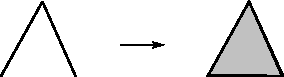
\includegraphics[scale=0.3]{Figures/2HornComb.pdf}
\item $H_{comb}(\ord{3})$ is \includegraphics[scale=0.3]{Figures/3HornComb.pdf}
\end{itemize}
\end{Example}

From the description in \autoref{Waldhausen} it is clear how $S$ extends to these objects. Altogether after applying $S$ and the transfer \autoref{VectTransfer} to $\Vect$ $\ord{1}$ goes to the space of functions on the isomorphism classes of objects of $\CCC$, and $\ord{n}$ goes to its $n^{th}$ tensor power presented as functions on isomorphism classes of $n$-tuples of objects.

\subsubsection{\texorpdfstring{$H_{comb}$}{Hcomb} on arrows}

Let $X \xrightarrow{f} Y$ be a map in $\OrdSet$. We want to associate to it a correspondence in $\sset^{op}$.

Let $y\in Y$ and denote $X_y$ the preimage of $y$ under $f$. Similarly to the above, we get an imbedding $\aug{X_y}$ in $\aug{X}$. Denote the sub-simplicial set generated by these imbeddings for all $y$ by $H_{comb}(f)$. Then we have a natural correspondence \[
H_{comb}(X) \rightarrow{} H_{comb}(f) \leftarrow H_{comb}(Y)
\]

\begin{Example}
The multiplication is the image of the map $\ord{2} \to \ord{1}$, and on the level of $H_{comb}$ this map goes to 
\[
\includegraphics[scale=0.5]{Figures/2MultComb.pdf}
\]
$S^{ext}$ then sends the middle object to the short exact sequences, and the maps to restriction to the endpoints or middle respectively. In all after applying transfer we get the usual multiplication in the Hall algebra.
\end{Example}

%%%%%%%%%%%%%%%%%%%%%%%%%%%%%%%%%%%%%

\subsubsection{\texorpdfstring{$H_{comb}$}{Hcomb} on squares}

Given a square in $\OrdSet$
\[
\stik{1}{
X \ar{r}{f} \ar{d}{g} \& Y \ar{d}{h}\\
Z \ar{r}{k} \& W
}
\]
Similarly to what we did with arrows, we have a map $X\xrightarrow{\alpha}W$ and we then construct the square of correspondences

\[
\stik{1}{
H_{comb}(X) \ar{r} \ar{d} \& H_{comb}(f) \ar{d}{}\& H_{comb}(Y) \ar{l} \ar{d} \\
H_{comb}(g) \ar{r} \& H_{comb}(\alpha) \& H_{comb}(h) \ar{l}{} \\
H_{comb}(Z) \ar{u} \ar{r} \& H_{comb}(k) \ar{u} \& H_{comb}(W) \ar{l} \ar{u}
}
\]

\begin{Example}
\label{AssocInSset}
The associator is the image of the square in $\OrdSet$ \[
\stik{1}{
\ord{3} \ar{r} \ar{d} \& \ord{2} \ar{d} \\
\ord{2} \ar{r} \& \ord{1}
}
\]

Its image under $H_{comb}$ is
\[
\includegraphics[scale=0.8]{Figures/AssocInSset.pdf}
\]

Note that in order to get associative multiplication after applying transfer construction from \autoref{transfer}, the extended $S$ construction should take the upper right and lower left squares to homotopy pullback squares. This is precisely equivalent to the 2-Segal conditions on $S_3,S_2,S_1$ from \cite{KapranovDyckerhoff}. i.e. that the induced maps
\begin{align*}
    S_{\{0123\}} &\to S_{\{013\}}\times_{S_{\{13\}}}S_{\{123\}}\\
    S_{\{0123\}} &\to S_{\{023\}}\times_{S_{\{02\}}}S_{\{012\}}
\end{align*}
are weak equivalences.
\end{Example}


%%%%%%%%%%%%%%%%%%%%%%%%%%%%%%%%%%%%


\section{Extending the algebra structure}
\label{Extension}
First we define a replacement for $\sset$ which is needed when extending the multiplication.

\begin{Definition}
Let $\DLat$ be the category of finite distributive lattices. The objects of interest to us in $\DLat$ are $\aug{X}$ for $X$ a finite grid poset (see \autoref{22case}) or a disjoint union of finite grids.

Define $\lSet$ to be the category of presheaves on $\DLat$.
\end{Definition}

Our goal in this section is to extend $H_{comb}$ to a functor $\OrdSet\otimes\OrdSet\to\Corr(\lSet^{op})$ and the Waldhausen construction to a functor $\lSet^{op}\to\Spaces$. Here by $\otimes$ we mean the Gray tensor of categories. All together we get an extension of $H_{geom}$ to a functor $\OrdSet\otimes\OrdSet\to\Corr(\Spaces)$
%%%%%%%%%%%%%%%%%%%%%%%%%%%%%%%%%%%%%%%%%%%
%%%%%%%%%%%%%%%%%%%%%%%%%%%%%%%%%%%%%%%%%%%

\subsection{Extension of \texorpdfstring{$H_{comb}$}{Hcomb}}
We explain the basics of the extension which will appear in detail in \cite{GeometricHallAlgebra2}.

\subsubsection{On objects}
An object of $\OrdSet\otimes\OrdSet$ is just a pair of objects $(X,Y)$ of $\OrdSet$. We consider first the grid poset $X\times Y$, and similarly to the construction in \autoref{HcombObjects} we note that for every \emph{level set} $(X\times Y)_d$ of the grid (i.e. the vertices at distance $d$ from the origin) we have an imbedding $\aug{(X\times Y)_d}$ in $\aug{X\times Y}$ and we define $H_{comb}(X,Y)$ to be the sub-$\lSet$ generated by the images of these imbeddings.

\begin{Example}
$H_{comb}(\ord{2},\ord{2})$ corresponds to the picture
\[
\includegraphics{Figures/squareHcombObject.pdf}
\]
\end{Example}
 where the right diagram is the poset $\aug{\ord{2}\times\ord{2}}$

\subsubsection{On arrows}
\label{HallCombArrows}
The arrows of $\OrdSet\otimes\OrdSet$ are generated by pairs of maps $(X,Y)\xrightarrow{f,g}(Z,W)$, where one of $(f,g)$ is the identity.

These generating arrows can be thought of as projections of grids. So suppose $P\xrightarrow{f} Q$ is such a projection. We want to construct a correspondence \[
\stik{1}{
H_{comb}(P) \ar{r}{s} \& X \& \ar{l}{p} H_{comb}(Q)
}
\]
We have a natural candidate for $X$: For any $d$, we consider the preimage of the level set $f^{-1}(Q_d)\subset P$, and in the same way as above we have an imbedding $\aug{f^{-1}(Q_d)}\to \aug{P}$. We let $X:=H_{comb}(f)$ be the sub-$\lSet$ generated by these images. An easy check shows that the map $\aug{Q}\xrightarrow{\aug{f}}\aug{P}$ lands in $H_{comb}(f)$ so defines the map $p$.

\textbf{Problem}: There is no natural map $H_{comb}(P)\to H_{comb}(f)$.

\textbf{Proposed solution}: We consider all intersections $f^{-1}(Q_d)\cap P_{d'}$ and the imbeddings of their augmentations in $\aug{P}$ and call what is generated $\overline{H_{comb}(f)}$. We now have a diagram\[
\stik{1}{
H_{comb}(P) \&\ar{l}{w} \overline{H_{comb}(f)} \ar{r}{s} \& H_{comb}(f) \& \ar{l}{p} H_{comb}(Q)
}
\]

\textbf{Why is this reasonable?} The maps $w$ go to an equivalence of stacks under $S$, so this can be considered as a localization.

\begin{Example}
\label{splitComb}
Consider the map $P=\ord{2}\times\ord{2}\xrightarrow{f}\ord{2}\times\ord{1}=Q$. It corresponds to the picture
\[
\includegraphics[scale=0.8]{Figures/squareHcombArrow.pdf}
\]
\end{Example}
In \autoref{splitWald} we explain in detail where the parts of this picture go under the extended Waldhausen construction.

\subsubsection{On squares}
\label{HCombSquares}
We start by giving the example of the square
\[
\stik{1}{
(\ord{2},\ord{2}) \ar{d}{} \ar{r}{} \& (\ord{2},\ord{1}) \ar{d}{} \\
(\ord{1},\ord{2}) \ar{r}{} \& (\ord{1},\ord{1})
}
\]
which goes to the Hopf relation.

It corresponds to the commutative diagram
\[
\includegraphics[scale=0.8]{Figures/HallHopfComb.pdf}
\]

From this example it should be clear how to write the image of a general square as a diagram in $\lSet$. The only issue is what kind of object this should be considered as. Our idea is that this should be considered as a square in the double category of correspondences in the localization double category of $\lSet$ at some class of "weak equivalences". We plan to explore this further in a future work.

For the purposes of this article however, all we need are constructions of certain squares and cubes and we verify the parts of the functoriality that we need locally.

%%%%%%%%%%%%%%%%%%%%%%%%%%%%%%%%%%%%%%%%%%%
%%%%%%%%%%%%%%%%%%%%%%%%%%%%%%%%%%%%%%%%%%%

\subsection{Extension of the Waldhausen construction}
\label{ExtWaldhausen}
Note that the $S$ construction from \autoref{Waldhausen} extends verbatim to the category $\POSet$ of finite posets. 

Note that also the augmentation functor extends to $\POSet\to \POSet^{op}$ by setting \[
\aug{X}=\Hom_{\POSet}(X,0\to 1)
\]

In fact all the posets that appear as augmentations in our picture are distributive lattices, so we think of $S$ as being defined on $\DLat$, and we claim that it naturally extends to $\lSet$. This depends on the behaviour of $S$ with respect to limits/colimits, along the lines of the 2-Segal property from \cite{KapranovDyckerhoff}.

\begin{Remark}
The category of presheaves on $\DLat$ appears in other contexts, for example as a framework for homotopy type theory in \cite{cubicalHott}.
\end{Remark}

%%%%%%%%%%%%%%%%%%%%%%%%%%%%%%%%%%%%%%%
%%%%%%%%%%%%%%%%%%%%%%%%%%%%%%%%%%%%%%
\subsubsection{The image of the square}
\label{22case}
Let $X=\aug{\ord{2}\times\ord{2}}$. This case plays a central role in our computation of the braiding.

%For simplicity we consider $\CCC$ to be (the $\infty$-derived category of) $\Vect$.

We start with a square
\[
\stik{1}{
1 \ar{r} \ar{d} \& 2 \ar{d}\\
3 \ar{r} \& 4
}
\]
 and consider its augmentation, i.e. all maps to $0\to 1$. If we denote by $M_T$ the map that sends the vertices in $T$ to $0$, then we see that $X$ is the poset

\[
\stik{1}{
{} \& {} \& M_{\{1,3\}}\ar{dr} \ar{drr} \& {} \& {} \\
M_{\{1,2,3,4\}} \ar{r} \ar{urr} \ar{drr} \& M_{\{1,2,3\}} \ar{ur} \ar{dr} \& {} \& M_{\{1\}} \ar{r} \& M_{\emptyset} \\
{} \& {} \& M_{\{1,2\}} \ar{ur} \ar{urr} \& {} \& {}
}
\]

Note that the top and bottom rows are the embeddings of $\aug{\ord{2}}$ coming from the projections from $\ord{2}\times\ord{2}$ to $\ord{2}$.

For the next step, recall that under Waldhausen construction the category that gets associated to \[
0\to 1 \to 2 = \aug{\ord{2}}
\]
is the category of short exact sequences
\[
0\to V_{01}\to V_{02}\to V_{12} \to 0
\]
For convenience, let us relabel the vertices of $X$ as

\begin{equation}
\label{augmentedSquare}
\stik{1}{
{} \& {} \& v\ar{dr} \ar{drr} \& {} \& {} \\
S \ar{r} \ar{urr} \ar{drr} \& 1 \ar{ur} \ar{dr} \& {} \& 2 \ar{r} \& T \\
{} \& {} \& h \ar{ur} \ar{urr} \& {} \& {}
}
\end{equation}
Then just by considering the sub-posets isomorphic to $\aug{\ord{2}}$, we see that an object of $S_X\CCC$ must contain a system of short exact sequences
\[
\nnstik{1}{
{S1} \ar{rr} \ar{dd}\& {} \& {Sv} \ar{dd} \ar{rr} \& {} \& {1v}\\
{} \& {} \&{} \& {h2} \ar{dr}\\
{Sh} \ar{rr} \ar{dd}\& {} \& {ST} \ar{dd} \ar{rr} \& {} \& {hT} \ar{dr} \\
{} \& {v2} \ar{dr} \&{} \&{} \& {} \& {2T}\\
{1h} \& {} \& {vT} \ar{dr} \& {} \& {} \\
{} \& {} \&{} \& {2T} \ar[equal]{uurr}
}
\]
(where labels $\alpha\beta$ denote the corresponding map $(0\to 1)\to X$ and colinear terms in the diagram form a short exact sequence)

Further analysing $\grid{X}$ we see that a map $\grid(X)\to \CCC$ contains pullback squares of the form
\[
\stik{1}{
0 \ar{r} \ar{d} \& 0\ar{d}\\
1v \ar{r} \& h2
}
\stik{1}{}
\stik{1}{
0 \ar{r} \ar{d} \& 0\ar{d}\\
1h \ar{r} \& v2
}
\]
 which gives us isomorphisms $1v\xrightarrow{\sim} h2$ and $v2\xrightarrow{\sim} 1h$.
 
In all we see that $S_X\CCC$ is equivalent to the category of grids
\[
\nnstik{1}{
{S1} \ar{rr} \ar{dd}\& {} \& {Sv} \ar{dd} \ar{rr} \& {} \& {1v} \ar{dd}\\
{} \& {} \&{} \& {} \\
{Sh} \ar{rr} \ar{dd}\& {} \& {ST} \ar{dd} \ar{rr} \& {} \& {hT} \ar{dd} \\
{} \& {}  \&{} \&{} \& {} \& {}\\
{1h} \ar{rr} \& {} \& {vT} \ar{rr} \& {} \& {2T}
}
\]


%%%%%%%%%%%%%%%%%%%%%%%%%%%%%%%%%%%%%%%
%%%%%%%%%%%%%%%%%%%%%%%%%%%%%%%%%%%%%%

\subsubsection{\autoref{splitComb} revisited}
\label{splitWald}

We now explain what the extended Waldhausen construction does to the diagram 
\[
\includegraphics[scale=0.8]{Figures/squareHcombArrow.pdf}
\]

The three rightmost objects correspond to the picture
\[
\includegraphics{Figures/HallHopfDoubleMult.pdf}
\]

Let us now consider the leftmost object and write it as a union of lattices, using the notation in \autoref{augmentedSquare}
\[
\stik{1}{
{} \& {} \& v\ar{dr} \& {} \& {} \\
S \ar{r}   \& 1 \ar{ur} \ar{dr} \& {} \& 2 \ar{r} \& T \\
{} \& {} \& h \ar{ur}  \& {} \& {}
}
\]

Repeating the relevant parts of the computation following \autoref{augmentedSquare}, we see that the Waldhausen construction sends this to the stack consisting of triples:
\begin{itemize}
    \item An object $S1$
    \item An object $2T$
    \item A diagram
    \[
    \nnstik{1}{
{}  \& {} \& {1v} \ar{dd} \ar{ddrr}[above,sloped]{\sim} \& {} \& {} \\
{} \& {} \&{} \& {} \\
{1h} \ar{rr} \ar{ddrr}[above,sloped]{\sim} \& {} \& {12} \ar{dd} \ar{rr} \& {} \& {h2}  \\
{} \& {}  \&{} \&{} \& {} \& {}\\
{}  \& {} \& {v2} \& {} \& {}
}
    \]
    where the row and column are short exact sequences
\end{itemize}

The leftmost map is then just the assignment to the quadruple of objects $(S1,1v,v2,2T)$ which can easily be seen to be an equivalence.


\subsection{Braided monoidal categories}
\label{DefnBraiding}
Conventionally one defines a braided monoidal category to be a monoidal category equipped with an additional natural isomorphism \[\gamma_{x,y}: \xymatrix{x \otimes y \ar[r]^{\sim} & y \otimes x}\] satisfying the so-called hexagon identities. 
In their foundational work on braided monoidal categories, Joyal and Street gave an equivalent way to define such structures \cite{Joyal-StreetBTC}. Namely, a braided monoidal category is equivalently a monoid object in the monoidal $2$-category $\mathbf{Mon}$. This $2$-category has objects monoidal categories, $1$-morphisms monoidal functors and $2$-morphisms monoidal natural transformation. The Cartesian product endows it with a monoidal structure. %We call such structures {\em doubly monoidal categories}
As this is the notion of braiding which we shall use throughout this paper we will now unpack the Joyal and Street definition.

\begin{Definition}
A braided monoidal category is the monoidal category \\$(\CCC, \otimes,\monunit, \alpha,\lambda, \rho)$ endowed with the following additional data:

\begin{enumerate}
    \item a functor $\mu: \CCC \times \CCC \to \CCC$;
    \item an isomorphism $\epsilon: \monunit \to \mu(\monunit,\monunit)$;
    \item a natural isomorphism
    \begin{equation}
        \stik{1}{
                \CCC^{\times 4} \ar{r}{\mu\times\mu} \ar{d}{\overline{\otimes}^2} \& \CCC^{\times 2} \ar{d}{\otimes}  \ar[Rightarrow, shorten <=1em,shorten >=1em]{dl}{\beta} \\
                \CCC^{\times 2} \ar{r}{\mu} \& \CCC
                }
    \end{equation}
    where $\overline{\otimes}^2$ is the induced monoidal structure on $\CCC \times \CCC$.
    \item natural isomorphisms $\varrho: \mu(-,\monunit) \Rightarrow \Id$ and $\Lambda: \mu(\monunit,-) \Rightarrow \Id$.
   
\end{enumerate}

 This data must make the following diagrams commute
    
    \lena{Make this cube look presentable as a separate equation. Write all the arrows for now. This is the 2-morphism inverse of the cube we wrote.}
   
   \begin{equation}%top-bottom,front-back,left-right
   \label{braidingcube}
\stik{2}{
{} \& {\CCC^4} \ar{rr}[name=topback,above]{\mu^2} \ar{dd}[name=backleft,xshift=-1pc,yshift=1pc]{\overline{\otimes}^2} \& {} \& {\CCC^2} \ar{dd}{\otimes}\\
{\CCC^6} \ar[crossing over]{rr}[name=topfront,below,xshift=1.5pc]{\mu^3}\ar{dd}[name=frontleft,below,xshift=-1.2pc,yshift=.4pc]{\overline{\otimes}^2 \times \Id^2} \ar{ur}[name=topleft,above, xshift=-.5pc]{\Id^2 \times \overline{\otimes}^2} \& {} \& {\CCC^3} \ar{dd}[name=frontright,xshift=-2.2pc,yshift=1.3pc]{\otimes\times \Id} \ar{ur}[name=topright,below,xshift=.4pc]{\Id\times \otimes} \& {}\\
{} \& {\CCC^2} \ar{rr}[xshift=.2pc]{\mu} \& {} \& {\CCC}\\
{\CCC^4} \ar{rr}[name=bottomfront,below]{\overline{\otimes}^2} \ar{ur}[name=bottomleft,sloped,yshift=-0.2pc]{} \& {} \& {\CCC^2} \ar{ur}[below]{\otimes}
\arrow[Rightarrow,to path={(topright) to[bend left] (topback)}]{}{\beta\times \Id_\mu}%may be wrong
\arrow[Rightarrow,to path={(frontright) to[bend right] (bottomfront)}]{}{\Id_\mu \times \beta}%may be wrong
\arrow[Rightarrow,crossing over,to path={(frontright) to[bend right] (topright)}]{}[below,xshift=.1pc]{\alpha}
\arrow[Rightarrow,to path={(bottomfront) to[bend right] (bottomleft)}]{}{\beta}
\arrow[Rightarrow,to path={(bottomleft) to[bend left] (backleft)}]{}{\overline{\alpha}^2}
\arrow[Rightarrow,to path={(topback) to[bend left] (backleft)}]{}{\beta}
\latearrow{commutative diagrams/crossing over}{2-3}{4-3}{}
\latearrow{commutative diagrams/crossing over}{2-1}{2-3}{}
}
\end{equation}
    
\[
\stik{1}{
                \otimes  (\mu \times \monunit) \ar[Rightarrow]{r}{\otimes (\mu \times \epsilon)} \ar[Rightarrow]{d}{\rho \mu} \& \otimes \mu^2 (\Id^2 \times \monunit^2) \ar[Rightarrow]{d}{\beta (\Id^2 \times \monunit^2)}  \\
                \mu\ar[Leftarrow]{r}{\mu \overline{\rho}^2} \& \mu \overline{\otimes}^2(\Id^2\times\monunit^2)
                } \]
                
\[
\stik{1}{
                \otimes (\monunit \times \mu) \ar[Rightarrow]{r}{\otimes (\epsilon \times \mu)} \ar[Rightarrow] {d}{\lambda \mu} \& \otimes \mu^2 (\monunit^2\times\Id^2) \ar[Rightarrow]{d}{\beta(\monunit^2\times\Id^2)}   \\
                \mu \ar[Leftarrow]{r}{\mu \overline{\lambda}^2} \& \mu \overline{\otimes}^2 (\monunit^2\times\Id^2)
                }\] 
                
\end{Definition}

%What about when C is linear? Should do everything in terms of \boxtimes and such. \lena{No, just say it carries over to this setting}

A monoidal category $(\CCC, \otimes,\monunit, \alpha,\lambda, \rho)$ with braiding $\gamma$ can be endowed with the above structure by defining $\beta = \Id\otimes \gamma \otimes \Id$, $\varrho = r^{-1}$ and $\Lambda = \lambda^{-1}$. Conversely, given the above structure on $\CCC$ one associates the braiding 
\begin{equation}
\label{ExtractBraiding}
\gamma = (\varrho \otimes \Lambda)^{-1} \circ \beta^{-1} \circ \mu(\rho,\lambda)^{-1} \circ \mu(\lambda,\rho) \circ \beta \circ (\Lambda \otimes \varrho). 
\end{equation}
These constructions extend to yield equivalences between the $2$-categories of braided monoidal categories and monoid objects in $\Mon$.


%\begin{Remark}
%The equivalence between these two definitions of a braided monoidal category is an instance of Dunn additivity for the $E_n$ operads \cite{Dunn}. The conventional definition says that a braided monoidal category is an algebra over the {\em parenthesized braid operad}, which is an $E_2$-operad in groupoids ***citation?***\lena{if true, citation is not needed}. The definition we use throughout this paper is that of an $E_1$-algebra in the category of $E_1$-algebras. The $n=2$ case of Dunn additivity, namely that $E_2$-alg$\ \simeq E_1$-alg$(E_1$-alg$)$, is the desired equivalence.
%\end{Remark}


\section{The braiding in the Hall algebra}
\label{BraidingHallAlgebra}
Here we explain how the extended Waldhausen construction produces a braiding.

Given a category $\CCC$ \adam{satisfying...} we construct the geometric Hall algebra $H_{geom}$ of $\CCC$ as in \autoref{GeneralHall} and compose it with $T^C$ from \autoref{CatTransfer} to get a functor $H_{\CCC}:\AugOrdSet\otimes\AugOrdSet\to\LinCat$. Denote $\HH:=H_\CCC(\ord{1})$.

The restriction of $H_{\CCC}$ to $\{1\}\otimes\AugOrdSet$ gives us a monoidal structure on $\HH$.

\begin{Theorem}
$H_\CCC$ induces a braiding on $\HH$.
\end{Theorem}

\begin{Example}
\label{VectHallExample}
For $\CCC=\Vect_\field$, $H_{\CCC}(\ord{1})\cong\bigoplus \Rep(\GL(n,\field))$
\end{Example}

Consider the image under $H_{geom}$ of the square in $\AugOrdSet\otimes\AugOrdSet$
\begin{equation}
\label{HopfSquare}
\stik{1}{
(\ord{2},\ord{2}) \ar{d}{} \ar{r}{} \& (\ord{2},\ord{1}) \ar{d}{} \\
(\ord{1},\ord{2}) \ar{r}{} \& (\ord{1},\ord{1})
}
\end{equation}

The image of this square under $H_{geom}$ is a square with a 2-morphism. It can be described pictorially as follows:

If we present the correspondence 
\[
\stik{1}{
{} \& S_2 \ar{dl}[above]{end} \ar{dr}{mid} \& {} \\
S_1\times S_1 \& {} \& S_1
}
\]
from \autoref{HallAlgebra} which gives the multiplication in the Hall algebra as the picture
\[
\includegraphics{Figures/HallMultPictorial.pdf}
\]

Then the image of the square is
\[
\includegraphics{Figures/HallHopfPictorial.pdf}
\]
The stack in the center of this square giving the 2-morphism is a grid of exact sequences with the obvious projections. We show how to get this square below in \autoref{Extension}.

Applying $T^C$, this gives a 2-morphism
\[
\stik{1}{
    \HH^{\otimes 4} \ar{r}{} \ar{d}{} \& \HH^{\otimes 2} \ar{d}{} \ar[Rightarrow, shorten <=1em,shorten >=1em]{dl}{}\\
    \HH^{\otimes 2} \ar{r}{} \& \HH
}
\]

If we restrict to objects of the form $1\otimes A\otimes B \otimes 1$ this gives a morphism $c_{A,B}:m(A,B)\to m(B,A)$ which is a candidate for a braiding.

\begin{Proposition}
\label{Thm:braiding}
$c_{A,B}$ defines a braiding on $\HH$
\end{Proposition}

The rest of this section is a sketch for a proof of \autoref{Thm:braiding}.
A rigorous treatment will be given in \cite{GeometricHallAlgebra2} where this result will follow from a more general result about the extended combinatorial Hall algebra construction.

As discussed in \autoref{BraidingGeneral}, we need to show that the cube \autoref{HexagonCube} constructed from the braiding and the associator, is commutative.

This cube is the image of the cube in $\AugOrdSet\otimes\AugOrdSet$:
\begin{equation}
\label{braidingcubeInDelta}
\stik{1}{
 \& (\ord{2},\ord{2}) \ar{rr} \ar{dd} \& {} \& (\ord{2},\ord{1}) \ar{dd}\\
(\ord{3},\ord{2}) \ar[crossing over]{rr} \ar{dd} \ar{ur} \& {} \& (\ord{3},\ord{1}) \ar{dd} \ar{ur} \& {}\\
{} \& (\ord{1},\ord{2}) \ar{rr} \& {} \& (\ord{1},\ord{1})\\
(\ord{2},\ord{2}) \ar{rr} \ar{ur} \& {} \& (\ord{2},\ord{1}) \ar{ur}
\latearrow{commutative diagrams/crossing over}{2-3}{4-3}{}
}
\end{equation}

We shall show that its image commutes already on the level of $H_{geo}$. That is, $H_{geo}$ produces for us a cube of correspondences, and in order for its image under $T^C$ to commute it is sufficient to show that the cubes in its upper-right-back and lower-left-front corners are pullback cubes (see \autoref{CorrCubeCommute}). Our main technical tool will be \autoref{PullbackCubeLemma}.

Let's consider first the lower-left-front cube. 

\begin{Claim}
\label{Lem:LeftFace}
Its left face is a pullback square
\end{Claim}

The underlying reason for this is that the left face of the original cube \autoref{braidingcubeInDelta} is the tensor of the associator square with itself.

Using this, and \autoref{PullbackCubeLemma}, we only need to prove that the right face is a pullback to get that the cube is a pullback.

A similar argument for the upper-right-back cube leads us to another inner square that we need to show is a pullback. In both cases these squares turn out to come from associator squares for the geometric Hall algebra associated to the category of short exact sequences in our original category. They are exactly the two squares that are pullbacks and correspond to the 2-Segal condition, as discussed in \cite[\S 4.5]{GeometricHallAlgebra1}.

\subsection{Recovering the braiding of Joyal and Street}

Here we consider the case $\CCC=\Vect_\field$. As noted in \autoref{VectHallExample}, in this case $\HH\cong\bigoplus \Rep(\GL(n,\field))$. More precisely, $H_{geom}(\ord{1})$ is the stack of vector spaces, so $\HH$ is really naturally the category of representations of the $\field$ points of this groupoid, which is what is called the category of linear species in \cite{Joyal-StreetGLn}.

\subsubsection{The monoidal structure}

The monoidal structure is given by $H_\CCC(\ord{2}\to\ord{1})$. Since $H_{geom}(\ord{2})$ is the stack of pairs of vector spaces, we have a canonical identification $H_\CCC(2)\cong\HH\otimes\HH$. Then, considering the diagram \autoref{HallMultCorrespondence} and using \autoref{GroupoidRep}, the monoidal structure $m$ is then given by the formula (for $\Phi,\Psi\in\HH$)
\[
m(\Phi,\Psi)(V)=\bigoplus_{[U\to V\to W]}\Phi(U)\otimes\Psi(W)
\]

where the sum goes over the isomorphism classes of the 2-fiber of the groupoid of short exact sequences in $\Vect_\field$ over the underlying groupoid of $\Vect_\field$ with respect to the map $mid$. A simple computation shows that this is in bijection with the set of subspaces $U\subseteq V$ so this is the same monoidal structure considered in \cite{Joyal-StreetGLn}.

\subsubsection{The braiding}

First consider the map of stacks $i:H_{geom}(\ord{2})\to H_{geom}(\ord{4})$ which sends a pair of vector spaces $(U,V)$ to the quadruple of vector spaces $(0,U,V,0)$.

We note that $T^C(i)$ implements the imbedding $\HH\otimes\HH\to\HH^{\otimes 4}, A\otimes B\mapsto \monunit\otimes A\otimes B \otimes \monunit$.

So in order to compute the braiding we need to apply $T^C$ to the diagram 
\[
\input{Figures/HallBraidPictorial.tex}
\]

This is the same as computing the 2-morphism in the square, but replacing all stacks with the ones where the upper-left and lower-right red dots correspond to the 0 object. This gives rise to the diagram

\[
\includegraphics{Figures/HallBraidPictorialReduced.pdf}
\]

Noting that a short exact sequence starting or ending with 0 is just an isomorphism, this reduces to the following correspondence of correspondences:
\[
\stik{1}{
{} \& S_2 \ar{dl}[above]{end} \ar{dr}{mid} \& {} \\
S_1\times S_1 \& E \ar{u}{vert} \ar{d}{hor} \& S_1\\
{} \& S_2 \ar{ul}[below]{end^{op}} \ar{ur}[below]{mid} \& {}
}
\]

where $E$ is the groupoid of diagrams of the form
\[
\stik{1}{
    {} \& U \ar{d} \ar{r}{\sim} \& U' \ar{d}[above,sloped]{\sim} \\
    W \ar{r}{} \ar{d}[above,sloped]{\sim} \& V \ar{r}{} \ar{d}{} \& U'' \\
    W' \ar{r}{\sim} \& W''
}
\]

with the horizontal and vertical mid lines being short exact sequences.

The isomorphism classes of the fiber of $E$ over $(U\to V\to W)\in S_2$ are in bijection with the set of subspaces in $V$ complementary to $U$. Using this, and \autoref{GroupoidRep}, we can compute that the 2-morphism is
\begin{align*}
    m(\Phi,\Psi)(V)&=\bigoplus_{U\subseteq V}\Phi(U)\otimes\Psi(V/U) \\
    &\xrightarrow{\epsilon} \bigoplus_{U\subseteq V}\bigoplus_{W\subseteq V,U\oplus W=V} \Phi(U)\otimes\Psi(V/U) \\
    &\xrightarrow{\alpha} \bigoplus_{U\subseteq V}\bigoplus_{W\subseteq V,U\oplus W=V} \Phi(V/W)\otimes\Psi(W) \\
    &\xrightarrow{\eta} \bigoplus_{W\subseteq V} \Phi(V/W)\otimes\Psi(W) \\
    &\cong m(\Psi,\Phi)(V)
\end{align*}

with $\epsilon,\eta$ being the obvious diagonal and codiagonal maps, and $\alpha$ induced by the canonical isomorphisms $U\cong V/W,V/U\cong W$.

Up to reordering the terms in the tensor product, this is exactly the braiding of \cite{Joyal-StreetGLn}.

\subsection{Braiding cube commutes}
In this section we show that the braiding cube \autoref{bradingcube} given by the extended Waldhausen construction always commutes.

The source for this cube is the following cube in $\OrdSet\otimes\OrdSet$ (described in \cite[\S3.4]{GGSSH}):
\[
C=\left(\stik{0.8}{
 \& \ord{3} \ar{rr} \ar{dd} \& {} \& \ord{2} \ar{dd}\\
\ord{3} \ar[crossing over]{rr} \ar{dd} \ar[equal]{ur} \& {} \& \ord{2} \ar{dd} \ar[equal]{ur}\& {}\\
{} \& \ord{2} \ar{rr} \& {} \& \ord{1}\\
\ord{2} \ar{rr} \ar[equal]{ur} \& {} \& \ord{1} \ar[equal]{ur}
\latearrow{commutative diagrams/crossing over}{2-3}{4-3}{}
}
,
\stik{0.8}{
 \& \ord{1} \ar[equal]{rr} \ar[equal]{dd} \& {} \& \ord{1} \ar[equal]{dd}\\
\ord{2} \ar[crossing over,equal]{rr} \ar[equal]{dd} \ar{ur} \& {} \& \ord{2} \ar[equal]{dd} \ar{ur}\& {}\\
{} \& \ord{1} \ar[equal]{rr} \& {} \& \ord{1}\\
\ord{2} \ar[equal]{rr} \ar{ur} \& {} \& \ord{2} \ar{ur}
\latearrow{commutative diagrams/crossing over,commutative diagrams/equal}{2-3}{4-3}{}
}
\right)
\]
and it's image is a cube of spans in stacks, i.e. a $2\times 2 \times 2$ grid of cubes. To show that the image in categories is commutative, we need to show that the upper-right-back and lower-left-front cubes are pullbacks.

Using \cite[Lemma A.2]{GeometricHallAlgebra1} we need to show that two opposing faces in each cube are pullbacks.

Consider first the upper-right-back cube. Looking at the back face of $C$ we see that its back face is the upper-right square of the image of the associator square, which is a pullback as discussed in \cite{GeometricHallAlgebra1} (this is equivalent to part of the 2-Segal condition).

Therefore, we only need to show that its front face is a pullback. Let us consider the square in $\lSet$ giving rise to it:
\[
\stik{1}{
 \aug{\ord{2}\times\ord{2}}\sqcup\aug{\ord{2}} \dar \& \aug{\ord{2}}\sqcup\aug{\ord{2}} \lar \dar\\
 \aug{\ord{3}\times\ord{2}} \& \aug{\ord{2}\times\ord{2}} \lar
}
\]

The image of this in stacks, in pictorial terms (as in \autoref{BraidingHallAlgebra}), is:
\[
\includegraphics{Figures/HallBraidCubeURB-F.pdf}
\]

which is clearly a pullback square. The argument for the lower-left-front cube is almost identical.

\section{Transfer theories}
In this section we outline two kinds of \emph{transfer theories}: The first  shows how to recover the usual Ringel-Hall algebra from our geometric Hall algebra construction and the second transfers the structure of the geometric Hall algebra to the world of linear categories. In particular using it we
recover the monoidal structure and the braiding on $\bigoplus_n \Rep(\GL(n,\FF_q))$ and \lena{other example?}

\subsection{Transfer to $\Vect$}
\label{VectTransfer}
\lena{Explain how 2-morphisms in $\Corr{\Spaces}$ give equalities}
This construction is based on a functor from the 1-category of correspondences of groupoids to $\Vect$ described in \cite[\S8.2]{KapranovDyckerhoff}. 

A stack $X$ over $\field$ is sent to the vector space of finitely supported functions on the set $\pi_0(X(\field))$ (i.e. the isomorphism classes of $X(\field)$) which we denote $\Func(X)$.

Given a correspondence $X \xleftarrow{s} Y \xrightarrow{p} Z$ we first send it to the correspondence of groupoids $X(\field) \xleftarrow{s} Y(\field) \xrightarrow{p} Z(\field)$ and then to the map $\Func(X) \to \Func(Z)$ given by $p_!s^*$. This assumes some restrictions on $s$ and $p$ (see \cite[\S 2]{Dyckerhoff}) which are always satisfied in the cases we consider. 

It follows immediately from \cite[Proposition 2.17]{Dyckerhoff} that this assignment is a transfer theory to $\Vect$.

Applying this transfer to $H_{geo}$ recovers the usual Hall algebra.
\subsection{Linear categories}
\label{LinCatTransfer}
Let $X$ be a groupoid and define $\Trans(X)$ to be the category of finitely supported representations of the groupoid $X(\FF_q)$ in $\Vect_\CC$. Using the pushforward defined in \autoref{GroupoidRep} we see that $\Trans$ is naturally a functor and for any $f:X\to Y$, $\Trans(f)$ has a biadjoint with explicit adjunctions. This means that for any square of correspondences we can produce a 2-morphism.




\section{Transfer to linear categories}
\label{Transferv2}

In this section we shall define a symmetric monoidal functor from the bicategory of iterated correspondences of (locally finite) groupoids to the bicategory of linear categories. The functor we write is a slight generalization of the {\em $2$-linearization} functor of Morton **CITE**, in that we extend the domain of definition from finite groupoids to locally finite groupoids.

The source of the functor is the symmetric monoidal bicategory of iterated correspondences of locally finite groupoids, $\Corr_2^\times$. The objects of this bicategory are the locally finite groupoids. A $1$-morphism from an object $\GG$ to an object $\GG'$ is a correspondence, that is, a diagram 
\begin{equation*}
    \stik{1}{ 
    \& \HH \ar[rd] \ar[ld] \& \\
    \GG \& \& \GG',}
\end{equation*}
wherein both functors are finite. Finally, a $2$-morphism is an equivalence class of correspondences of correspondences, that is, an equivalence class of diagrams
\begin{equation*}
    \stik{1}{ \& \& \HH \ar{rrd} \ar{lld} \ar[Rightarrow, shorten <=1em,shorten >=2em]{ldd} \ar[Rightarrow, shorten <=1em,shorten >=2em]{rdd} \& \& \\
    \GG \& \& \mathcal{I} \ar{u} \ar{d}    \& \& \GG'.\\
     \& \ \& \HH' \ar{rru} \ar{llu} \& \ \& } %This sucks
\end{equation*}
wherein all functors are finite. Two such diagrams are equivalent when ***BLAH BLAH*** **CITE MORTON**.

\begin{Remark}
Locally finite groupoids and finite functors between them form an $\infty$-category $\Spaces$ having finite limits. In **CITE** Haugseng defines a symmetric monoidal $(\infty,2)$-category of iterated correspondences in $\CCC$ for any $\infty$-category $\CCC$ having finite limits. The symmetric monoidal bicategory $\Corr_2^\times$ is the homotopy bicategory of Haugseng's $(\infty,2)$-category of iterated correspondences in $\Spaces$.
\end{Remark}




\section{Review of linear categories}
\label{LinCats}

Throughout this paper, the term {\em linear category} will refer to a semisimple abelian category compatibly enriched in $\Vect$ such that every strictly descending chain of subobjects is finite. A functor between linear categories will always be assumed to be additive, right exact and compatible with the $\Vect$-enrichment. 
\begin{Remark}
We assume these conditions to ensure that the {\em Deligne-Kelly product} exists \cite{Franco}. Namely, for any two linear categories $L$ and $L'$ there is a universal linear category $L \boxtimes L'$ with a bilinear functor $L \times L' \to L \boxtimes L'$ 
\end{Remark}

In this paper we will only consider a specific class of linear categories and functors between them arising from groupoid representations. 

\begin{Definition}
A groupoid $\GG$ is said to be {\em locally finite} if $|\Hom(i,i')| < \infty$ for all objects $i$ and $i'$ of $\GG$. 
\end{Definition}

Each such groupoid is equivalent to one which is specified by two pieces of data: namely, a set $I$ indexing the isomorphism classes of objects and, for each $i \in I$, a finite group $G_i$ of automorphisms of $i$. We write such a groupoid as $\GG \simeq \coprod_{i \in I} G_i$.


\begin{Definition}
A groupoid is {\em finite} if it is locally finite and has finitely many isomorphism classes of objects. A functor $F: \GG \to \HH$ is {\em finite} if for each object $j$ of $\HH$, the (homotopy) fibre, $F^{-1}(j)$ is a finite groupoid.
\end{Definition}

Writing $\GG \simeq \coprod_{i \in I} G_i$ and $\HH \simeq \coprod_{j \in J} H_j$, a functor $F: \GG \to \HH$ is equivalent to a function $f:I \to J$ and, for each $i \in I$, a group homomorphism $F_i: G_i \to H_{f(i)}$. Written this way $F$ is finite if and only if $|f^{-1}(j)| < \infty$ for each $j \in J$ and $F_i$ has finite kernel and cokernel for each $i \in I$. (\cite{KapranovDyckerhoff} 8.2.3).

\begin{Remark}
Note that when $\GG$ and $\HH$ are locally finite the latter condition is automatically satisfied.
\end{Remark} 

\begin{Definition}
The category of representations of a groupoid $\GG$, $\RR(\GG)$, is the category of finitely supported functors $\GG \to \Vect$. That is, $\RR(\GG)$ is the full subcategory of $\Fun(\GG,\Vect)$ consisting of those functors which send all but finitely many isomorphism classes of objects in $\GG$ to the $0$ vector space. 
\end{Definition}

All linear categories considered in this paper will be of the form $\RR(\GG)$ for $\GG$ locally finite. Writing $\GG \simeq \coprod_{i \in I} G_i$ one has that $\RR(\GG) \simeq \oplus_{i \in I} \Rep(G_i)$, which are evidently linear in our sense. Further, one can readily check that for $\GG$ and $\GG'$ locally finite, $\RR(\GG) \boxtimes \RR(\GG') \simeq \RR(\GG \times \GG')$. 

\begin{Proposition}
(Morton, ***CITE***) For $F: \GG \to \HH$ a finite functor between locally finite groupoids the restriction functor $F^*: \RR(\HH) \to \RR(\GG)$ admits an ambidextrous adjoint $F_*: \RR(\GG) \to \RR(\HH)$.
\end{Proposition}
\begin{proof}
 First, note that since $F$ is finite the left and right adjoints to $F^*$ are given, respectively, by left and right Kan extension. Writing $\GG \simeq \coprod_{i \in I} G_i$ and $\HH\simeq \coprod_{j \in J} H_j$, one can compute, using the pointwise formulas for Kan extensions, that these adjoints are given by
\begin{align}
 F_* \ \rho(j) &= \bigoplus_{i \ : \ f(i)=j} \Hom_{\CC[G_i]}\left(\CC[H_j], \rho(i) \right) \nonumber \\
 F_! \ \rho(j) &= \bigoplus_{i \ : \ f(i)=j} \CC[H_j] \otimes_{\CC[G_i]} \rho(i) \nonumber.
\end{align}
 

Next, for $f:G \to H$ a group homomorphism between finite groups and $V$ a left $G$-module the map
 \begin{align}
   \Hom_{\CC[G]}\left(\CC[H], V \right) &\to \CC[H] \otimes_{\CC[G]} V \nonumber \\
  \phi &\mapsto  \frac{1}{|G|} \sum_{h \in H} h^{-1} \otimes \phi(h) \nonumber %The centering on this is less than ideal
 \end{align}
is an isomorphism of left $H$-modules. This assembles into a natural isomorphism $ F_* \simeq F_!$.

\end{proof}

The units and counits which witness $F_*$ being both left and right adjoint to $F^*$ can be readily computed. As we shall need them in the sequel, we record here  the unit for the right adjunction, $\eta_F^R: \Id_{\RR(\HH)} \Rightarrow F_* F^*$, and the counit for the left adjunction, $\eps_F^L: F_*F^* \Rightarrow \Id_{\RR(\HH)}$. For each $\rho \in \RR(\HH)$ and object $j$ of $\HH$ these natural transformations have components
\begin{align}
\label{unitexp}
\eta_F^R(\rho)(j): \rho(j) \ &\to \bigoplus_{i \ : \ f(i)=j} \CC[H_j] \otimes_{\CC[G_i]} \rho(j) \\ \nonumber
v \ &\mapsto \bigoplus_{i \ : \ f(i)=j} \frac{1}{| G_i |} \sum_{h \in H_j} h \otimes h^{-1} \cdot v
\end{align}
and
\begin{align}
\label{counitexp}
\eps_F^L(\rho)(j): \bigoplus_{i \ : \ f(i)=j} \CC[H_j] \otimes_{\CC[G_i]} \rho(j) \ &\to \rho(j) \\ \nonumber
\bigoplus_{i \ : \ f(i)=j} h_j \otimes v \ &\mapsto \sum_{i \ : \ f(i)=j} h_j \cdot v.
\end{align}






%\section{The Braiding is an isomorphism}
\label{BraidingIso}

%Obviously this title needs to change. The contents of this section should appear in the paper, but the exact way in which it happens depends on broader content aspects.

The goal of this section is to prove that the braiding introduced in Section ***REF*** is in fact an isomorphism. To begin, we reduce the braiding square ***REF*** to a form which is amenable to direct calculation.

Given non-negative integers $n_1, \ldots, n_k$ with $n_1 + \cdots n_k = n$ we define the following subgroups of $\GLn$: 
\begin{itemize}
\item $\GL_{n_1,\ldots,n_k} := \GL_{n_1} \times \cdots \times \GL_{n_k}$, the block diagonal subgroup;
\item  $P_{n_1,\ldots,n_k}$, the parabolic subgroup corresponding to the flag 
\begin{equation*}
    0 \subset \CC^{n_1} \subset \CC^{n_1 + n_2} \subset\cdots \subset \CC^{n_1 + \cdots n_k}.
\end{equation*}
\item $K_{n_1,\ldots, n_k}$, the kernel of the surjection 
\begin{equation*}
\pi_{n_1,\ldots, n_k}:\xymatrix{P_{n_1,\ldots, n_k} \ar@{->>}[r] & \GL_{n_1,\ldots, n_k}}
\end{equation*}
sending a flag-preserving automorphism to the induced automorphism of the relevant quotient spaces. One therefore has that 
\begin{equation*}
    P_{n_1,\ldots, n_k} = K_{n_1,\ldots, n_k} \rtimes \GL_{n_1,\ldots, n_k};
\end{equation*}
 
\item  $\PP_{n_1, n_2, n_3, n_4}$, the intersection of the parabolic subgroups $P_{n_1, n_2, n_3, n_4}$ and $P_{n_1, n_3, n_2, n_4}$.
\end{itemize}

 
\begin{Proposition}
The square defining the braiding ***REF*** is equivalent to the correspondence
\begin{equation}
    \xymatrix{ & \ar@{->>}[ld]_-\pi \coprod_{a,b,c,d} P_{a,b,c,d} \ar@{^{(}->}[rd]^-i & \\
    \coprod_{a,b,c,d} \GL_{a,b,c,d} & \coprod_{a,b,c,d} \PP_{a,b,c,d} \ar@{^{(}->}[u]^-I \ar@{^{(}->}[d]_-{\tilde{I}} & \coprod_{n} \GLn, \\
    & \ar@{->>}[lu]^-{\tilde{\pi}} \coprod_{a,b,c,d} P_{a,c,b,d}\ar@{^{(}->}[ru]_-{\tilde{i}} & }
\end{equation}
where $I$, $i$, $\tilde{I}$ and $\tilde{i}$ are given by the obvious subgroup inclusions, and $\pi$ and $\tilde{\pi}$ are given by the surjections $\pi_{a,b,c,d}$.
\end{Proposition}
\begin{proof}
Composing the outer edges of the square yields the correspondence

****** NICE FIGURE WITH H's, I's AND GRID ******

Therefore it suffices to determine skeletal forms for the groupoid ***I***, ***H*** and ****GRID*** and the induced functors between them. Further, note that the skeletons of each of these groupoids have object set given by $4$-tuples of non-negative integers. We proceed by fixing such a $4$-tuple $a,b,c,d$ and determining the corresponding automorphism groups.

For the groupoid ***I***, the automorphism group is the intersection of the parabolics $P_{a,b,a+b+c+d}$ and $P_{c,c+d} \subset \GL_{c+d} \subset \GL_{a+b+c+d}$ inside $\GL_{a+b+c+d}$. This is exactly the parabolic $P_{a,b,c,d}$. The same argument, {\em mutatis mutandi}, proves the claim for the groupoid ***H***.

Finally, for the groupoid ***GRID***, any automorphism must fix both the ***I***-shaped and ***H***-shaped subdiagrams, so the automorphism group must be a subgroup of $P_{a,b,c,d} \cap P_{a,c,b,d}$. One readily verifies that {\em every} element of this intersection defines an automorphism of the grid. %Not great write-up. 
\end{proof}

The braiding $\beta$ is therefore given by the following composition
\begin{equation}
    \xymatrix{i_* \pi^* \ar@{=>}[r]^-{\eta^R_I} & i_* I_* I^* \pi^* \ar@{=}[r] & \tilde{i}_* \tilde{I}_* \tilde{I}^* \tilde{\pi}^* \ar@{=>}[r]^-{\eps_{\tilde{I}}^L} & \tilde{i}_* \tilde{\pi}^*}.
\end{equation}
To show that $\beta$ is a natural isomorphism it suffices to show that for each $4$-tuple $a,b,c,d$, and each $\rho \in \Rep(\GL_{a,b,c,d})$ the component $\beta(\rho)$ is an isomorphism.



\begin{Lemma}
The components of the braiding $\beta$ corresponding to a representation $\rho \in \Rep(\GL_{a,b,c,d})$ are given by
\begin{align}
\CC[\GL_n]\otimes_{\CC[P_{a,b,c,d}]} \rho &\to \CC[\GL_n] \otimes_{\CC[P_{a,c,b,d}]} \rho \\ \nonumber
\gamma \otimes v &\mapsto \frac{\left|\GL_{a,b,c,d}\right|}{\left| \PP_{a,b,c,d} \right|} \sum_{k \in K_{a,b,c,d}} \gamma k \otimes v. \nonumber
\end{align}
\end{Lemma}
\begin{proof}
By equation \eqref{unitexp}, $\eta^R_I$ sends $\gamma \otimes v$ to the element of $\CC[\GL_n] \otimes_{\CC[P_{a,b,c,d}]} \left( \CC[P_{a,b,c,d}] \otimes_{\CC[\PP_{a,b,c,d}]} \rho\right)$  given by %doesn't look nice
\begin{equation*}
\frac{1}{\left| \PP_{a,b,c,d} \right|} \sum_{p \in P_{a,b,c,d}}\gamma \otimes p \otimes p^{-1} \cdot v = \frac{1}{\left| \PP_{a,b,c,d} \right|} \sum_{p \in P_{a,b,c,d}}\gamma \otimes p \otimes \pi_{a,b,c,d}(p)^{-1} v.
\end{equation*}
Since $P_{a,b,c,d} = K_{a,b,c,d} \rtimes \GL_{a,b,c,d}$ every $p \in P_{a,b,c,d}$ can be uniquely written as $p=k g$ where $k \in K_{a,b,c,d}$ and $g \in \GL_{a,b,c,d}$ where $g = \pi_{a,b,c,d}(p)$. Therefore the image of $\gamma \otimes v$ is equal to
\begin{equation*}
 \frac{1}{\left| \PP_{a,b,c,d} \right|} \sum_{\substack{ k \in K_{a,b,c,d} \\ g \in \GL_{a,b,c,d}
 }}\gamma \otimes k g \otimes g^{-1} v = \frac{\left|\GL_{a,b,c,d}\right|}{\left| \PP_{a,b,c,d} \right|} \sum_{k \in K_{a,b,c,d}} \gamma k \otimes e \otimes v,
\end{equation*}
where we used that $\GL_{a,b,c,d} \subset \PP_{a,b,c,d}$ and $K_{a,b,c,d} \subset P_{a,b,c,d}$.

Applying the counit $\eps^L_{\tilde{I}}$ to the above expression yields by equation \eqref{counitexp} the claimed expression for the components of $\beta$.
\end{proof} 

\begin{Theorem}
The braiding $\beta$ is an isomorphism.
\end{Theorem}
\begin{proof}

\end{proof}

%\section{Localization}
\label{App:localization}
In \autoref{HallCombArrows} we propose that the maps appearing in the combinatorial Hall algebra construction should be in a kind of localization of $\lSet$. 

Here we describe this kind of structure more generally, and not very rigorously.

Let $\DDD$ be a category, and $W$ some class of "weak equivalences". As usual we denote maps in $W$ by $\xrightarrow{\sim}$. We construct a double category $\DDD_W$ as follows:
\begin{itemize}
    \item Objects are objects of $\DDD$.
    \item Morphisms $A$ to $B$ are diagrams of the form $A\xleftarrow{\sim}E\to B$.
    \item Squares are commutative diagrams of the form
    \[
   \stik{1}{
    A \& E \ar{l}[above,sloped]{\sim} \ar{r}{} \& B \\
    F \ar{u}[above,sloped]{\sim} \ar{d}{}\& Z \ar[leftarrow]{ul} \ar[leftarrow]{ur} \ar[leftarrow]{dl} \ar[leftarrow]{dr}[above,sloped]{\sim}\& G\ar{u}[above,sloped]{\sim} \ar{d} \\
    C \& H \ar{l}[above,sloped]{\sim} \ar{r} \& D \\
    }
    \]
\end{itemize}

\begin{Remark}
If a functor $\DDD\xrightarrow{\phi}\CCC$ maps $W$ to isomorphisms, then it factors through $\DDD_W$ with the functor $\DDD_W\xrightarrow{\phi_W}\CCC$ being defined by
\[
A\xleftarrow{\stackrel{\alpha}{\sim}}E\xrightarrow{f} B\mapsto \phi(A)\xrightarrow{\phi(f)\phi(\alpha)^{-1}}\phi(B)
\]
It is then easy to check that squares go to commutative squares.
\end{Remark}

\subsection{Some conditions on \texorpdfstring{$W$}{W}}
For $\DDD_W$ as described to be closed on composition of morphisms and squares we can require the following of $W$:
\begin{itemize}
    \item $W$ is stable under pullback and pushout by any morphism in $\DDD$.
    \item All morphisms in $W$ are epimorphisms in $\DDD$.
\end{itemize}

\subsection{Transfer}

If we have a transfer theory from $\DDD$ then it can be extended to a transfer from $\DDD_W$ in a straightforward way.

\subsection{Correspondences}

It is straightforward to extend the construction of $\Corr(\DDD)$ to get a double category $\Corr(\DDD_W)$ where we replace the commutative squares by squares in $\DDD_W$. 
This is the form of what we get in \autoref{HCombSquares}.

\subsection{Weak equivalences in \texorpdfstring{$\lSet$}{lSet}}

Currently we don't have a good description of what we would like to call weak equivalences in general in $\lSet$, but we have many examples, such as the one we saw above:

\[
\includegraphics{Figures/lSetEquivs.pdf}
\]

Most likely it would be helpful if this is part of a model structure on $\lSet$.

\section{Representations of groupoids}
\label{GroupoidRep}
In this section we recall some basic notions regarding representations of groupoids and give a convenient formula for the push forward functor.

\begin{Definition}
A \emph{representation} of a groupoid $G$ is a functor $G\to \Vect_{\field}$ which is non-zero only on finitely many connected components of $G$. Denote the category of representations of $G$ by $\Rep(G)$.
\end{Definition}

\begin{Definition}
\label{2Fiber}
Let $G\xrightarrow{p} H$ be a morphism of groupoids. Recall that the fiber of $p$ over $h\in H$ is the groupoid with objects $(g\in G, p(g)\xrightarrow{\sigma} h)$ and morphisms being $g\to g'$ which make everything commute. Denote the fiber $F_h$, and its canonical map to $G$ by $F_h\xrightarrow{i}G$. 
\end{Definition}
\begin{Definition}
Say that a morphism $G\xrightarrow{p} H$ of groupoids is \emph{finitary} if $F_h$ has finitely many isomorphism classes for every $h$. 
\end{Definition}

We have an obvious functor $p^*:\Rep(H)\to\Rep(G)$ given by precomposition.

\begin{Proposition}
$p^*$ has a bi-adjoint functor $p_*$
\end{Proposition}
\begin{proof}
Let $\rho\in\Rep(G)$ and $h\in H$. We give an explicit formula for $p_*(\rho)(h)$ using the fiber of $p$ over $h$.

Denote by $[F_h]$ the set of isomorphism classes of $F_h$, then the formula for the adjoint is
\begin{equation}
p_*(\rho)(h)=\bigoplus_{x\in [F_h]} \rho(i(x))\otimes_{\field [\Aut_{F_h}(x)]}\field
\end{equation}

(the tensoring with $\field$ is just taking co-invariants with respect to $\Aut_{F_h}(x)$).

To complete the description we need to explain how $p_*(\rho)$ acts on maps in $H$. So let $h\xrightarrow{\tau}h'$ be a map, which since $H$ is a groupoid must be an isomorphism. First, note that $\tau$ induces an equivalence $F_h\to F_{h'}$ by $(g, p(g)\xrightarrow{\sigma} h)\mapsto(g, p(g)\xrightarrow{\tau\circ\sigma} h') $. In particular it induces a bijection $[F_h]\to [F_{h'}]$ which we will also denote by $\tau$. The map $p_*(\rho)(h)\to p_*(\rho)(h')$ is then given by the maps $\rho(i(x))\to\rho(i(\tau(x)))$. It is straightforward to check that this is well defined, and functorial in $\rho$.

Now we need to give the unit and co-unit maps. Let us assume for simplicity that $p$ is faithful, and hence $\Aut_{F_h}(x)$ is trivial for all $x$. Let $\rho\in\Rep(G),\theta\in\Rep(H)$, then
\begin{eqnarray}
p_*p^*(\theta)(h)&=\bigoplus_{x\in [F_h]} \theta(p(i(x)))\cong \bigoplus_{x\in [F_h]} \theta(h)\\
p^*p_*(\rho)(g)&=p_*(\rho)(p(g))=\bigoplus_{x\in [F_{p(g)}]} \rho(i(x))
\end{eqnarray}

The maps $\Id\to p_*p^* \to \Id$ are just the diagonal and averaging maps. The maps $\Id\to p^*p_* \to \Id$ are partial diagonal and averaging maps, using the isomorphisms $i(x)\cong g$ lifting $p(i(x))\cong p(g)$, whenever the lift exists.
\end{proof}

\begin{appendices}
\section{Pullback cubes}

\begin{Definition}
\label{PullbackCube}
A commutative cube \[
\stik{1}{
 \& A \ar{rr} \ar{dd} \& {} \& B \ar{dd}\\
X \ar[crossing over]{rr} \ar{dd} \ar{ur} \& {} \& Y \ar{dd} \ar{ur} \& {}\\
{} \& C \ar{rr} \& {} \& D\\
Z \ar{rr} \ar{ur} \& {} \& W \ar{ur}
\latearrow{commutative diagrams/crossing over}{2-3}{4-3}{}
}
\]
is said to be a \emph{pullback} cube if it presents $X$ as the limit of the rest of the diagram. i.e. for any other commutative cube 
\[
\stik{1}{
 \& A \ar{rr} \ar{dd} \& {} \& B \ar{dd}\\
\widetilde{X} \ar[crossing over]{rr} \ar{dd} \ar{ur} \& {} \& Y \ar{dd} \ar{ur} \& {}\\
{} \& C \ar{rr} \& {} \& D\\
Z \ar{rr} \ar{ur} \& {} \& W \ar{ur}
\latearrow{commutative diagrams/crossing over}{2-3}{4-3}{}
}
\]
There exists a unique morphism $\widetilde{X}\to X$ making everything commute.
\end{Definition}

\begin{Lemma}
\label{PullbackCubeLemma}

For simplicity we will consider the 1-category case, as the proof works very similarly for 2-categories.

Consider a commutative cube in some category
\[
\stik{1}{
 \& A \ar{rr} \ar{dd} \& {} \& B \ar{dd}\\
X \ar[crossing over]{rr} \ar{dd} \ar{ur} \& {} \& Y \ar{dd} \ar{ur} \& {}\\
{} \& C \ar{rr} \& {} \& D\\
Z \ar{rr} \ar{ur} \& {} \& W \ar{ur}
\latearrow{commutative diagrams/crossing over}{2-3}{4-3}{}
}
\]
And suppose that $ABCD$ is a pullback square, then $XYZW$ is a pullback square if and only if the whole cube is a pullback cube.
\end{Lemma}

\begin{proof}
Assume $XYZW$ is a pullback square.

Consider another commutative cube 
\[
\stik{1}{
 \& A \ar{rr} \ar{dd} \& {} \& B \ar{dd}\\
\widetilde{X} \ar[crossing over]{rr} \ar{dd} \ar{ur} \& {} \& Y \ar{dd} \ar{ur} \& {}\\
{} \& C \ar{rr} \& {} \& D\\
Z \ar{rr} \ar{ur} \& {} \& W \ar{ur}
\latearrow{commutative diagrams/crossing over}{2-3}{4-3}{}
}
\]
We want to show that there is a unique map $\widetilde{X}\to X$ that makes everything commute.

Since $XYZW$ is a pullback square we have a unique map $\widetilde{X}\to X$ such that $\widetilde{X}Y=XY\circ\widetilde{X}X$ and $\widetilde{X}Z=XZ\circ\widetilde{X}X$.

we just need to show that $\widetilde{X}A=XA\circ\widetilde{X}X$. This follows because both sides are a map $\widetilde{X} \to A$ which make the diagram
\[
\stik{1}{
\widetilde{X} \ar{dr} \ar{drr} \ar{ddr} \\
{} \& A \ar{d} \ar{r}\& B \ar{d} \\
{} \& C \ar{r} \& D
}
\]
commute. Since we assumed $ABCD$ is a pullback such a map is unique.

Assume now that the cube is a pullback and consider a square \[
\stik{1}{
\widetilde{X} \ar{r} \ar{d} \& Y \ar{d} \\
Z \ar{r} \& W
}
\]
We want to show that there is a unique map $\widetilde{X}\to X$ which makes the diagram 
\[
\stik{1}{
\widetilde{X} \ar{dr} \ar{drr} \ar{ddr} \\
{} \& X \ar{d} \ar{r}\& Y \ar{d} \\
{} \& Z \ar{r} \& W
}
\]
commute.

The compositions $YB\circ\widetilde{X}Y$ and $ZC\circ\widetilde{X}Z$ fit in a commutative square 
\[
\stik{1}{
\widetilde{X} \ar{r} \ar{d} \& B \ar{d} \\
C \ar{r} \& D
}
\]
and so there is a map $\widetilde{X}\to A$ that makes everything commute, and since the cube is a pullback this gives us our desired map $\widetilde{X}\to X$.
\end{proof}
\end{appendices}
\printbibliography
\end{document}






































